% =====================================================
% CHAPITRE 2 : TESTS DE CHARGE ET INJECTION DE FAUTES
% =====================================================
\chapter{Tests de Charge et Injection de Fautes}
\label{chap:tests-chaos}

\section{Introduction}

Ce chapitre présente la méthodologie expérimentale complète de nos tests de chaos engineering. Nous combinons deux approches complémentaires : la génération de charge réaliste avec \textbf{Apache JMeter} pour simuler des utilisateurs réels, et l'injection de fautes contrôlées avec \textbf{Pumba} pour provoquer des défaillances ciblées sur l'infrastructure.

L'objectif est de mesurer la résilience du système sous conditions normales puis dégradées, en observant les métriques de performance (latence, débit, taux d'erreurs) et de disponibilité via les dashboards Grafana configurés au chapitre précédent.

\section{Tests de charge avec Apache JMeter}

\subsection{Présentation de JMeter}

Apache JMeter est un outil open-source de test de performance permettant de simuler des charges utilisateur sur des applications web. Il offre :
\begin{itemize}
    \item Simulation de multiples utilisateurs concurrents
    \item Support de protocoles variés (HTTP, HTTPS, REST, SOAP)
    \item Extraction et validation de données (JSON, XML)
    \item Génération de rapports de performance détaillés
    \item Scripting avec variables, boucles et conditions
\end{itemize}

\subsection{Scénarios de test développés}

Trois scénarios JMeter ont été développés pour couvrir différents niveaux de complexité et de charge :

\subsubsection{Test 1 : User Service Load Test}

\textbf{Objectif} : Valider la capacité du User Service à gérer des opérations de création d'utilisateurs et d'adresses sous charge modérée.

\textbf{Configuration} :
\begin{itemize}
    \item \textbf{Nombre d'utilisateurs virtuels} : 50
    \item \textbf{Ramp-up} : 30 secondes
    \item \textbf{Itérations} : 10 par utilisateur
\end{itemize}

\textbf{Scénario} :
\begin{enumerate}
    \item \textbf{Create User} : Création d'un utilisateur avec username, email et mot de passe uniques
    \item \textbf{Extract User ID} : Extraction de l'ID utilisateur créé via JSON Extractor
    \item \textbf{Create Address} : Création d'une adresse de livraison pour cet utilisateur
    \item \textbf{Get All Users} : Récupération de la liste complète des utilisateurs
    \item \textbf{Think Time} : Pause aléatoire entre 500ms et 1500ms
\end{enumerate}

\textbf{Assertions} :
\begin{itemize}
    \item Code HTTP 201 (Created) ou 409 (Conflict si doublon) pour Create User
    \item Code HTTP 200 (OK) pour Get All Users
\end{itemize}

\subsubsection{Test 2 : Product Service Load Test}

\textbf{Objectif} : Évaluer les performances du catalogue produits sous forte charge de consultation, simulant un pic de trafic e-commerce.

\textbf{Configuration} :
\begin{itemize}
    \item \textbf{Nombre d'utilisateurs virtuels} : 100
    \item \textbf{Ramp-up} : 60 secondes
    \item \textbf{Itérations} : 20 par utilisateur
\end{itemize}

\textbf{Scénario} :
\begin{enumerate}
    \item \textbf{Get All Products} : Récupération du catalogue complet
    \item \textbf{Search Products} : Recherche avec mot-clé aléatoire parmi : laptop, phone, book, shoes, gadget
    \item \textbf{Get Products by Category} : Filtrage par catégorie (ID aléatoire 1-4)
    \item \textbf{Get Product by ID} : Consultation détaillée d'un produit (ID aléatoire 1-5)
    \item \textbf{Think Time} : Pause aléatoire entre 200ms et 1000ms
\end{enumerate}

\textbf{Points d'attention} :
\begin{itemize}
    \item Ce test génère \textbf{2000 requêtes totales} (100 users × 20 iterations)
    \item Sollicitation intensive du Product Service et de la base de données
    \item Permet d'observer la dégradation progressive sous charge
\end{itemize}

\subsubsection{Test 3 : E2E Shopping Flow}

\textbf{Objectif} : Simuler un parcours complet d'achat (end-to-end) sollicitant l'ensemble des microservices de manière coordonnée.

\textbf{Configuration} :
\begin{itemize}
    \item \textbf{Nombre d'utilisateurs virtuels} : 20
    \item \textbf{Ramp-up} : 60 secondes
    \item \textbf{Itérations} : 5 par utilisateur
\end{itemize}

\textbf{Scénario détaillé} :
\begin{enumerate}
    \item \textbf{Get Users with Addresses} : Récupération d'un utilisateur avec ses adresses
    \begin{itemize}
        \item Extraction aléatoire d'un \texttt{USER\_ID} et \texttt{ADDRESS\_ID}
    \end{itemize}
    
    \item \textbf{Browse Products} : Navigation dans le catalogue
    \begin{itemize}
        \item Extraction d'un \texttt{PRODUCT\_ID} aléatoire
    \end{itemize}
    
    \item \textbf{View Product Details} : Consultation détaillée du produit sélectionné
    
    \item \textbf{Add to Cart (Loop 3×)} : Ajout de 3 produits au panier
    
    \item \textbf{View Cart} : Consultation du panier complet
    
    \item \textbf{Create Order} : Transformation du panier en commande
    \begin{itemize}
        \item Extraction de l'\texttt{ORDER\_ID} généré
    \end{itemize}
    
    \item \textbf{View Order Details} : Consultation de la commande créée
    
    \item \textbf{Think Time} : Pause aléatoire entre 1s et 3s
\end{enumerate}

Ce scénario E2E est particulièrement sensible aux pannes, car il sollicite l'ensemble des services de manière séquentielle.



\section{Injection de fautes avec Pumba}

\subsection{Présentation de Pumba}

\begin{figure}[H]
\centering
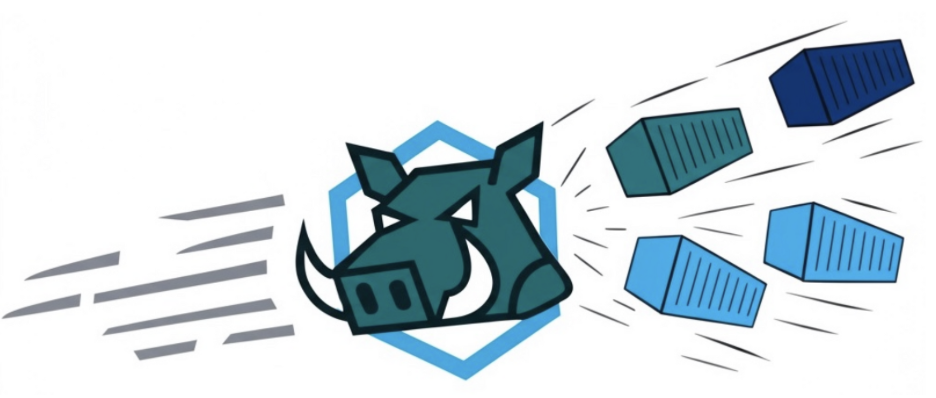
\includegraphics[width=0.6\textwidth]{images/Pumba.png}
\caption{Pumba}
\end{figure}

Pumba est un outil de chaos engineering spécialisé pour Docker, permettant d'injecter des fautes au niveau conteneur et réseau. Il s'interface directement avec l'API Docker pour manipuler les conteneurs en cours d'exécution.

\textbf{Capacités principales} :
\begin{itemize}
    \item \textbf{Stop/Kill} : Arrêt gracieux ou brutal de conteneurs
    \item \textbf{Pause/Unpause} : Gel temporaire d'un conteneur
    \item \textbf{Network Emulation (netem)} : Latence, perte de paquets, duplication, corruption
    \item \textbf{Stress} : Surcharge CPU/mémoire
\end{itemize}

\subsection{Configuration de l'environnement de test}

\subsubsection{Contexte et contraintes}

\begin{itemize}
    \item \textbf{Point d'entrée unique} : Spring Cloud Gateway 
    \item \textbf{Instances uniques} : Chaque service déployé en 1 seule réplica
    \item \textbf{Pas de politique de redémarrage} : \texttt{restart} non défini dans docker-compose.yml
    \item \textbf{Conséquence} : Une panne de conteneur = indisponibilité totale du service (SPOF)
\end{itemize}

\subsubsection{Cible des tests}

\begin{itemize}
    \item \textbf{Service cible} : \texttt{product-service}
    \item \textbf{Raison du choix} : Service le plus sollicité par les scénarios JMeter
    \item \textbf{Sélection Pumba} : Regex exacte \texttt{re2:\^{}product-service\$}
    \item \textbf{Réseau} : \texttt{ecommerce-network} (bridge)
    \item \textbf{Image TC} : \texttt{gaiadocker/iproute2} pour les règles \texttt{netem}
\end{itemize}

\subsection{Scénarios de pannes}

\subsubsection{Scénario 1 : Arrêt temporaire (Stop)}

\textbf{Objectif} : Simuler une maintenance planifiée ou un redémarrage gracieux du service.

\begin{lstlisting}[caption={Commande Pumba - Stop 30s}]
docker run -it --rm \
  -v /var/run/docker.sock:/var/run/docker.sock \
  --network ecommerce-network \
  gaiaadm/pumba:0.9.0 \
  stop --duration 30s --time 10s re2:^product-service$
\end{lstlisting}

\textbf{Paramètres} :
\begin{itemize}
    \item \texttt{--duration 30s} : Le conteneur reste arrêté pendant 30 secondes
    \item \texttt{--time 10s} : Délai avant l'injection (permet de démarrer JMeter d'abord)
\end{itemize}

\textbf{Comportement attendu} :
\begin{itemize}
    \item $t = 10s$ : Arrêt gracieux du conteneur (\texttt{SIGTERM})
    \item $t = 10s \rightarrow 40s$ : Product Service indisponible (30s downtime)
    \item $t = 40s$ : Redémarrage automatique du conteneur
    \item Disponibilité théorique : $\frac{270s}{300s} \times 100 = 90\%$ (sur fenêtre 5 min)
\end{itemize}

\textbf{Impact observé} :
\begin{itemize}
    \item Requêtes vers Product Service → erreurs 502/503/504 (Bad Gateway/Service Unavailable/Timeout)
    \item Services dépendants (Cart, Order, Review) → erreurs partielles ou complètes
    \item Métrique Grafana \texttt{up\{instance="product-service:8082"\}} → passe de 1 à 0 puis retour à 1
\end{itemize}

\subsubsection{Scénario 2 : Crash brutal (Kill)}

\textbf{Objectif} : Simuler un crash applicatif ou système (OOM, segfault, kernel panic).

\begin{lstlisting}[caption={Commande Pumba - Kill SIGTERM}]
docker run -it --rm \
  -v /var/run/docker.sock:/var/run/docker.sock \
  gaiaadm/pumba:0.9.0 \
  kill --signal SIGTERM re2:^product-service$
\end{lstlisting}

\begin{lstlisting}[caption={Commande Pumba - Kill SIGKILL (brutal)}]
docker run -it --rm \
  -v /var/run/docker.sock:/var/run/docker.sock \
  gaiaadm/pumba:0.9.0 \
  kill --signal SIGKILL re2:^product-service$
\end{lstlisting}

\textbf{Différence SIGTERM vs SIGKILL} :
\begin{itemize}
    \item \textbf{SIGTERM} : Signal gracieux, permet au processus de nettoyer les ressources (fermer connexions DB, flush logs)
    \item \textbf{SIGKILL} : Terminaison immédiate, aucun cleanup possible (simule un kill -9 ou perte d'alimentation)
\end{itemize}

\textbf{Comportement observé} :
\begin{itemize}
    \item Sans \texttt{restart: always} → Le conteneur reste DOWN indéfiniment
    \item Product Service indisponible jusqu'à intervention manuelle (\texttt{docker compose up -d})
    \item Disponibilité = 0\% après le kill
\end{itemize}

\subsubsection{Scénario 3 : Latence réseau (Netem Delay)}

\textbf{Objectif} : Simuler une dégradation réseau (congestion, distance géographique, routage sous-optimal).

\begin{lstlisting}[caption={Commande Pumba - Latence 500ms ±100ms}]
docker run -it --rm \
  -v /var/run/docker.sock:/var/run/docker.sock \
  --network ecommerce-network \
  gaiaadm/pumba:0.9.0 netem \
    --tc-image gaiadocker/iproute2 \
    --duration 2m delay \
      --time 500 --jitter 100 --distribution normal \
    re2:^product-service$
\end{lstlisting}

\textbf{Paramètres netem} :
\begin{itemize}
    \item \texttt{--time 500} : Délai moyen de 500ms ajouté à chaque paquet
    \item \texttt{--jitter 100} : Variation aléatoire de ±100ms
    \item \texttt{--distribution normal} : Distribution gaussienne du jitter
    \item \texttt{--duration 2m} : Injection active pendant 2 minutes
\end{itemize}

\textbf{Résultat} : Latence effective entre 400ms et 600ms (distribution normale).

\textbf{Impact observé} :
\begin{itemize}
    \item Latence p95 des requêtes HTTP → augmentation de 50-100ms à 600-700ms
    \item Timeout potentiels si RestTemplate configuré avec timeout < 700ms
    \item Débit (throughput) → diminution de 20-40\% due aux requêtes plus lentes
    \item Disponibilité → reste à 100\% (service répond, mais lentement)
\end{itemize}

\subsubsection{Scénario 4 : Perte de paquets (Netem Loss)}

\textbf{Objectif} : Simuler une connexion réseau instable (WiFi dégradé, réseau saturé).

\begin{lstlisting}[caption={Commande Pumba - Perte 20\% de paquets}]
docker run -it --rm \
  -v /var/run/docker.sock:/var/run/docker.sock \
  --network ecommerce-network \
  gaiaadm/pumba:0.9.0 netem \
    --tc-image gaiadocker/iproute2 \
    --duration 2m loss --percent 20 \
    re2:^product-service$
\end{lstlisting}

\textbf{Paramètres} :
\begin{itemize}
    \item \texttt{--percent 20} : 20\% des paquets réseau sont aléatoirement supprimés
    \item Effet cumulatif : requête HTTP nécessite plusieurs paquets (requête + réponse)
\end{itemize}

\textbf{Impact observé} :
\begin{itemize}
    \item Requêtes HTTP → certaines échouent directement (paquets perdus)
    \item Retransmissions TCP → augmentation de la latence (exponential backoff)
    \item Taux d'erreurs → 5-15\% de requêtes en échec
    \item Latence p95 → augmentation de 100-200ms due aux retransmissions
    \item Débit → diminution de 30-50\%
    \item Disponibilité apparente → 85-95\% (certaines requêtes passent)
\end{itemize}

\subsubsection{Scénario 5 : Chaos continu (micro-coupures périodiques)}

\textbf{Objectif} : Simuler des micro-instabilités réseau répétées (flapping network).

\begin{lstlisting}[caption={Commande Pumba - Cycles de latence 15s toutes les 30s}]
docker run -it --rm \
  -v /var/run/docker.sock:/var/run/docker.sock \
  gaiaadm/pumba:0.9.0 \
  --interval 30s --random netem \
    --tc-image gaiadocker/iproute2 \
    --duration 15s delay --time 200 \
    re2:^product-service$
\end{lstlisting}

\textbf{Paramètres} :
\begin{itemize}
    \item \texttt{--interval 30s} : Nouvelle injection toutes les 30 secondes
    \item \texttt{--duration 15s} : Chaque injection dure 15 secondes
    \item \texttt{--random} : Ajoute un délai aléatoire avant chaque injection
    \item \texttt{delay --time 200} : Latence de 200ms pendant les 15s actives
\end{itemize}

\textbf{Comportement} :
\begin{itemize}
    \item Cycle : 15s de latence → 15s normal → 15s latence → ...
    \item Crée des oscillations dans les métriques (pics de latence périodiques)
\end{itemize}

\textbf{Impact observé} :
\begin{itemize}
    \item Métriques Grafana → courbes en dents de scie (oscillations)
    \item Latence p95 → pics périodiques à 250-300ms
    \item Taux d'erreurs → pics légers pendant les fenêtres de latence
    \item Disponibilité → reste proche de 100\% mais avec dégradations intermittentes
\end{itemize}

\section{Protocole expérimental}

\subsection{Méthodologie générale}

Chaque test suit un protocole en trois phases pour mesurer l'impact des fautes :

\begin{figure}[H]
\centering
\begin{tikzpicture}[scale=0.8]
\draw[->] (0,0) -- (14,0) node[right] {Temps};
\draw[->] (0,0) -- (0,4) node[above] {Métriques};

% Baseline
\draw[thick, blue] (0,3) -- (5,3) node[midway, above] {Baseline};
\draw[dashed] (5,0) -- (5,4) node[above] {$t_1$};

% Chaos
\draw[thick, red] (5,3) -- (5,1.5) -- (7,1.5) -- (7,1) -- (10,1);
\node[red, above] at (7.5,1.5) {Injection};
\draw[dashed] (10,0) -- (10,4) node[above] {$t_2$};

% Recovery
\draw[thick, green!60!black] (10,1) -- (10.5,1.5) -- (11,2) -- (14,2.8);
\node[green!60!black, above] at (12,2.5) {Recovery};

\end{tikzpicture}
\caption{Chronologie expérimentale : Baseline → Chaos → Recovery}
\end{figure}

\textbf{Phase 1 : Baseline (5 minutes)} :
\begin{itemize}
    \item Système en fonctionnement normal
    \item Exécution du test JMeter pour établir les métriques de référence
    \item Observation : latence nominale, taux d'erreurs $\approx$ 0\%, débit stable
\end{itemize}

\textbf{Phase 2 : Chaos (2-5 minutes)} :
\begin{itemize}
    \item Injection de la faute Pumba (stop/kill/delay/loss)
    \item Poursuite de l'exécution JMeter (même charge)
    \item Observation : dégradation des métriques en temps réel
\end{itemize}

\textbf{Phase 3 : Recovery (5 minutes)} :
\begin{itemize}
    \item Fin de l'injection (Pumba se termine ou conteneur redémarre)
    \item Observation du retour à la normale
    \item Mesure : temps de récupération (recovery time)
\end{itemize}

\subsection{Matrice de tests}

\begin{table}[H]
\centering
\small
\begin{tabular}{lccc}
\toprule
\textbf{Scénario Pumba} & \textbf{Test JMeter} & \textbf{Durée Chaos} & \textbf{Durée Totale} \\
\midrule
Stop 30s & Product Load & 30s & ~10 min \\
Kill SIGTERM & Product Load & Indéfini & ~8 min \\
Kill SIGKILL & E2E Shopping & Indéfini & ~15 min \\
Delay 500ms & Product Load & 2 min & ~12 min \\
Loss 20\% & Product Load & 2 min & ~12 min \\
Chaos continu & E2E Shopping & 5 min & ~20 min \\
\bottomrule
\end{tabular}
\caption{Matrice des combinaisons test JMeter × scénario Pumba}
\end{table}

\subsection{Commandes d'exécution coordonnées}

\textbf{Terminal 1 - Démarrage JMeter} :
\begin{lstlisting}[caption={Lancement test JMeter en mode non-GUI}]
# Product Service Load Test
jmeter -n -t jmeter-tests/product-service-load-test.jmx

# E2E Shopping Flow
jmeter -n -t jmeter-tests/e2e-shopping-flow.jmx
\end{lstlisting}

\textbf{Terminal 2 - Injection Pumba (après 1 minute de baseline)} :
\begin{lstlisting}[caption={Injection de faute avec timing}]
# Attendre 60s pour baseline, puis injecter
sleep 60 && docker run -it --rm \
  -v /var/run/docker.sock:/var/run/docker.sock \
  --network ecommerce-network \
  gaiaadm/pumba:0.9.0 netem \
    --tc-image gaiadocker/iproute2 \
    --duration 2m delay --time 500 --jitter 100 \
    re2:^product-service$
\end{lstlisting}

\textbf{Terminal 3 - Surveillance Grafana} :
\begin{itemize}
    \item Ouvrir le dashboard "Product Service – Application \& Container"
    \item Activer l'auto-refresh (5s ou 10s)
    \item Ajouter des annotations manuelles aux moments clés :
    \begin{itemize}
        \item Annotation "Baseline Start" à $t_0$
        \item Annotation "Chaos Injection" à $t_1$ (commande Pumba lancée)
        \item Annotation "Chaos End" à $t_2$ (fin d'injection)
    \end{itemize}
\end{itemize}

\section*{Conclusion du chapitre}

Ce chapitre a présenté la méthodologie complète de nos expérimentations de chaos engineering. Nous avons détaillé :

\begin{itemize}
    \item \textbf{Trois scénarios JMeter} : User Load (50 users), Product Load (100 users), E2E Shopping (20 users)
    \item \textbf{Cinq types de pannes Pumba} : Stop, Kill (SIGTERM/SIGKILL), Delay, Loss, Chaos continu
    \item \textbf{Protocole expérimental} : Baseline → Chaos → Recovery avec captures Grafana annot